\documentclass[a4paper,12pt]{article}

\usepackage{cmap}		
\usepackage[utf8]{inputenc}			
\usepackage[english,russian]{babel}
\usepackage{framed}
\usepackage{hyperref}
\usepackage{amsmath}
\usepackage{amsfonts}
\usepackage[T2A]{fontenc}
\usepackage{graphicx}
\usepackage[colorinlistoftodos]{todonotes}
\usepackage{wrapfig}
\usepackage{lipsum}
\usepackage{color}
\usepackage{indentfirst}
\usepackage{times}
\usepackage{textcomp}
\usepackage{float}
\usepackage{listings}
\usepackage{xcolor}
\usepackage[T1]{fontenc}

\usepackage{morewrites}

\usepackage[pdf]{graphviz}
\usepackage{xpatch}
\makeatletter
\newcommand*{\addFileDependency}[1]{% argument=file name and extension
  \typeout{(#1)}
  \@addtofilelist{#1}
  \IfFileExists{#1}{}{\typeout{No file #1.}}
}
\makeatother
\xpretocmd{\digraph}{\addFileDependency{#2.dot}}{}{}

\usepackage[autosize]{dot2texi}
\usepackage{tikz}
\usetikzlibrary{shapes,arrows}

\newcommand{\HRule}{\rule{\linewidth}{0.5mm}}

\begin{document}

\begin{titlepage}
\begin{center}



% Upper part of the page. The '~' is needed because \\
% only works if a paragraph has started.
\textsc{\Large НАЦИОНАЛЬНЫЙ ИССЛЕДОВАТЕЛЬСКИЙ УНИВЕРСИТЕТ}\\
\textsc{\Large "МЭИ"}\\[1cm]


\includegraphics[width=0.8\textwidth]{img/logo.png}~\\[1cm]

\textsc{\Large Теоретические модели вычисления}\\[0.5cm]

% Title
\HRule \\[0.4cm]
{ \LARGE \bfseries ДЗ №3: Машины Тьюринга и квантовые вычисления \\[0.4cm] }

\HRule \\[1.5cm]

% Author and supervisor
\noindent
\begin{minipage}{0.4\textwidth}
\begin{flushleft} \large
\emph{Студент:}\\
Николаев \textsc{Ю.~С.}
\end{flushleft}
\end{minipage}%
\begin{minipage}{0.4\textwidth}
\begin{flushright} \large
\emph{GitHub:} \\
\href{https://github.com/NRU-MPEI-IMAI/tm-and-qc-nikolaevje}{@nikolaevje}
\end{flushright}
\end{minipage}

\vfill

% Bottom of the page
{\large Москва, 2022}

\end{center}
\end{titlepage}

\newpage
\tableofcontents

\newpage

\section{Машины Тьюринга}

\subsection{Операции с числами}

Реализуйте машины Тьюринга, которые позволяют выполнять следующие операции:
\begin{enumerate}
    \item Сложение двух унарных чисел (1 балла) [1\_1\_1.yml]
    
    \begin{center}
        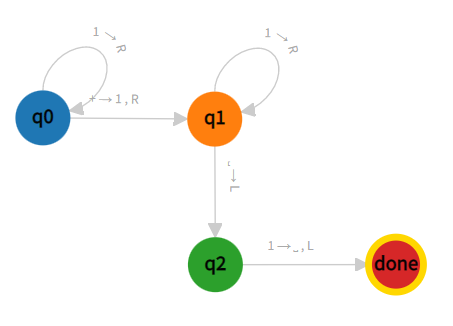
\includegraphics[scale=0.8]{img/1_1_1.png}
    \end{center}
    
    \item Умножение унарных чисел (1 балл) [1\_1\_2.yml]
    
    \begin{center}
        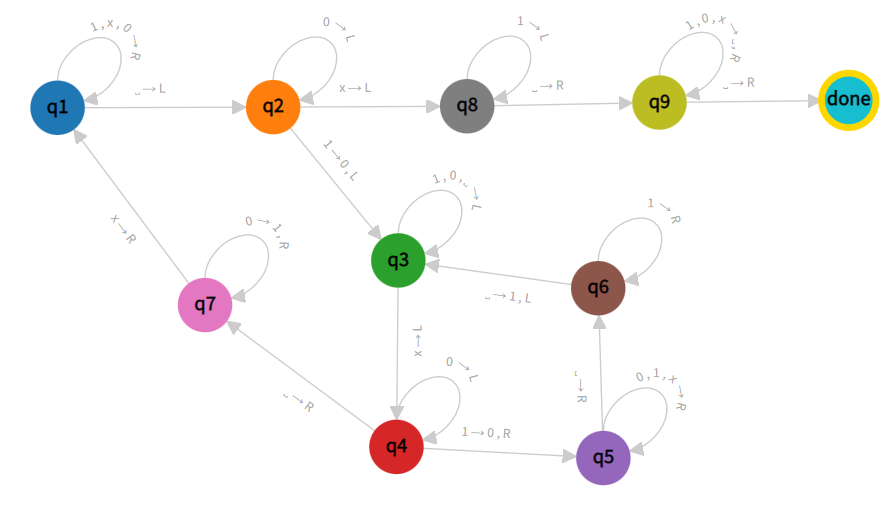
\includegraphics[scale=0.8]{img/1_1_2.png}
    \end{center}
\end{enumerate}


\subsection{Операции с языками и символами}

Реализуйте машины Тьюринга, которые позволяют выполнять следующие операции:
\begin{enumerate}
    \item Принадлежность к языку $L = \{ 0^n1^n2^n \}, n \ge 0$ (0.5 балла) [1\_2\_1.yml]
    
    \begin{center}
        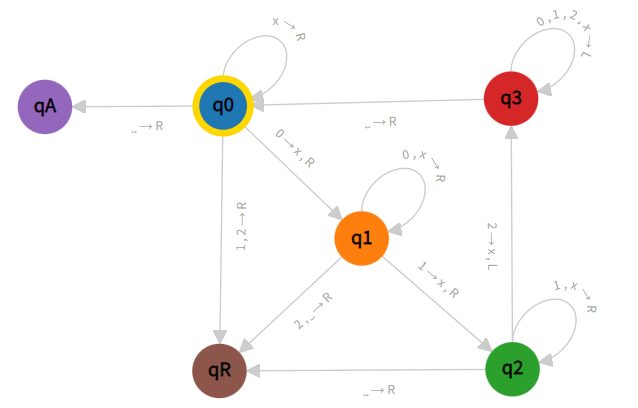
\includegraphics[scale=0.6]{img/1_2_1.png}
    \end{center}
    
    \item Проверка соблюдения правильности скобок в строке (минимум 3 вида скобок) (0.5 балла) [1\_2\_2.yml]
    
    \begin{center}
        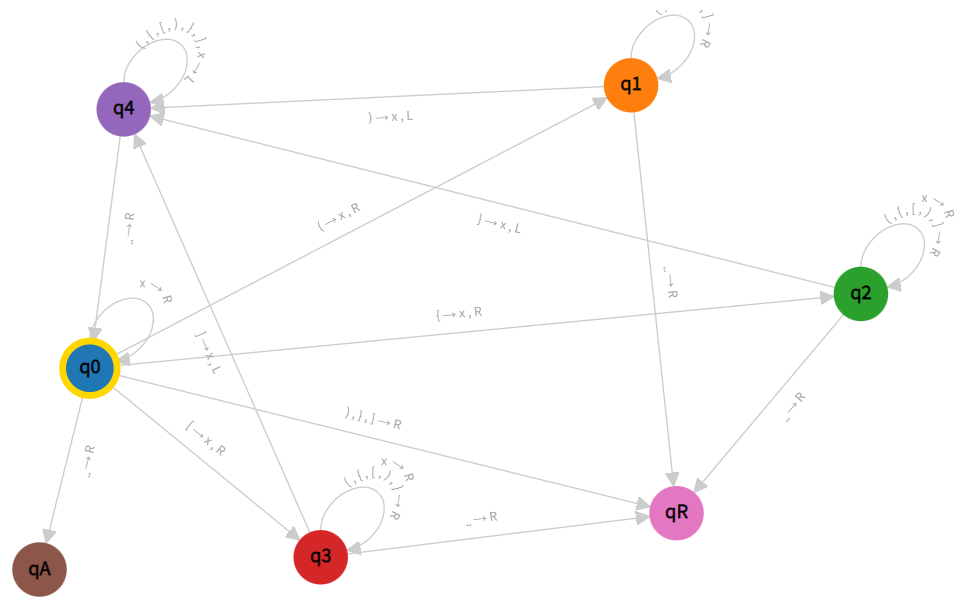
\includegraphics[scale=0.8]{img/1_2_2.png}
    \end{center}
    
    \item Поиск минимального по длине слова в строке (слова состоят из символов 1 и 0 и разделены пробелом) (1 балл)
    
    \begin{center}
        Это я не сделал, зато здесь будет котик
        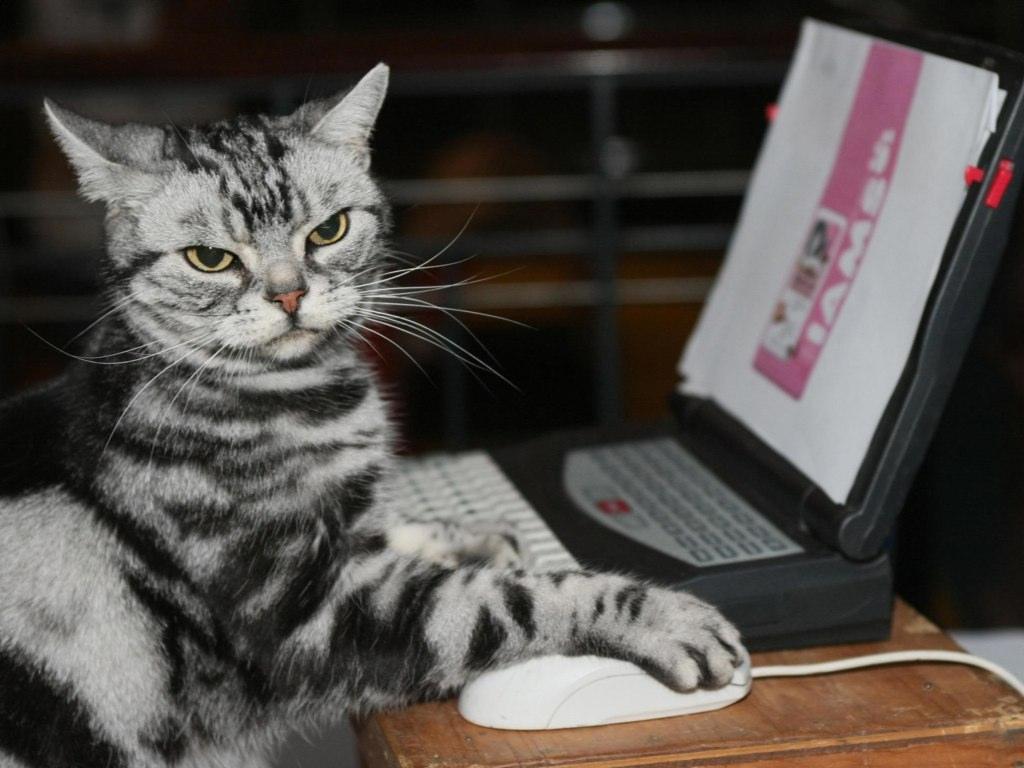
\includegraphics[scale=0.2]{img/1_2_3.jpg}
    \end{center}
\end{enumerate}


\section{Квантовые вычисления}

В качестве решения задачи надо предоставить схему алгоритма для частного случая при фиксированном количестве кубитов и фиксированных состояниях. 


\subsection{Генерация суперпозиций 1 (1 балл)}

Дано $N$ кубитов ($1 \le N \le 8$) в нулевом состоянии $\Ket{0\dots0}$. Также дана некоторая последовательность битов, которое задаёт ненулевое базисное состояние размера $N$. Задача получить суперпозицию нулевого состояния и заданного.

$$\Ket{S} = \frac{1}{\sqrt2}(\Ket{0\dots0} +\Ket{\psi})$$

То есть требуется реализовать операцию, которая принимает на вход:

\begin{enumerate}
    \item Массив кубитов $q_s$
    \item Массив битов $bits$ описывающих некоторое состояние $\Ket{\psi}$. Это массив имеет тот же самый размер, что и $qs$. Первый элемент этого массива равен $1$.
\end{enumerate}

Первые кубиты 1 и 0 - различны, применяем гейт Адамара. А дальше, если $bits[i] == 1$, то спутываем $i$-ый кубит с первым с помощью $CNOT$.

Например, $N = 3$, $bits = [1, 1, 1]$:

Тогда:

\begin{center}
    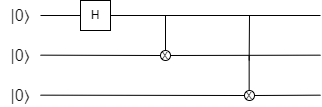
\includegraphics[scale=0.7]{img/3_1_1.png}
\end{center}

Код для $N = 1, 2, ..., 8$:
\begin{lstlisting}
namespace Solution {
        open Microsoft.Quantum.Primitive;
        open Microsoft.Quantum.Canon;
        operation Solve (qs : Qubit[], bits : Bool[]) : ()
        {
            body
            {
                H(qs[0]);
                for (i in 1..Length(qs) - 1)
                    if (bits[i])
                        CNOT(qs[0], qs[i]);
            }
        }
}
\end{lstlisting}

\begin{center}
    А дальше я не делал, зато выспался!

    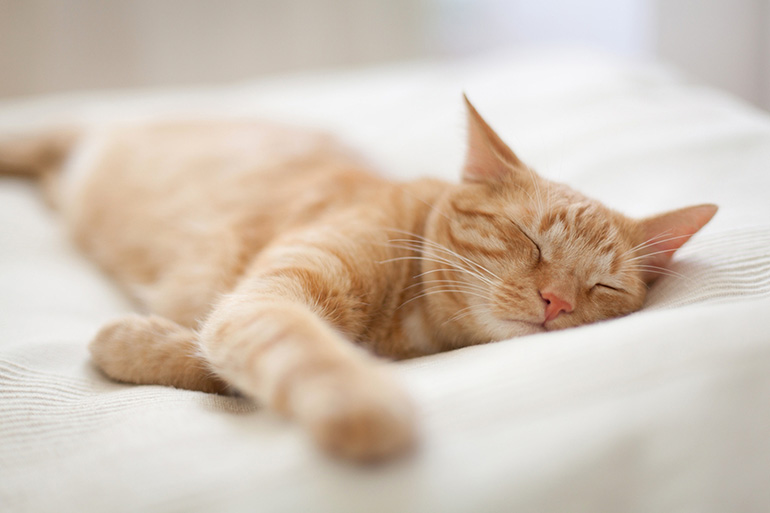
\includegraphics[scale=0.4]{img/cat_sleeps.jpg}
\end{center}

\end{document}

\usepackage[english,russian]{babel}